% KansasLava-AK.tex
\begin{hcarentry}{HERMIT}
\label{HERMIT}
\report{Andy Gill}%11/10
\participants{Andy Gill, Andrew Farmer, Ed~Komp, PostDoc (TBA)}
\status{active}
\makeheader

The Haskell Equational Reasoning Model-to-Implementation Tunnel
(HERMIT) is an NSF-funded project being run at KU to improving the
Applicability of Haskell-Hosted Semi-Formal Models to High Assurance
Development. Specifically, HERMIT will use the worker/wrapper
transformation, a Haskell-hosted DSL, and a new refinement UI to
perform rewrites directly on Haskell Core, the GHC internal
representation.

This project is a substantial case study into the application of
worker/wrapper on larger examples. In particular, we want to
demonstrate the equivalences between efficient Haskell programs, and
their clear, specification-style Haskell counterparts. In doing so,
there are several open problems, including refinement scripting and
management scaling issues, data representation and presentation
challenges, and understanding the theoretical boundaries of the
worker/wrapper transformation.

The project is expected to run through 2013, and will be released
open-source in due time.

\begin{center}
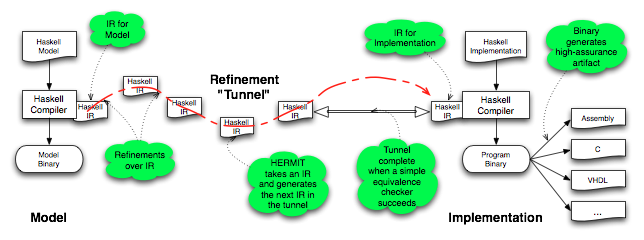
\includegraphics[width=1\textwidth]{html/HERMIT-tunnel.png}
\end{center}

\FurtherReading
  \url{http://www.ittc.ku.edu/csdl/fpg/Tools/HERMIT}
\end{hcarentry}
